\documentclass[10pt,twocolumn]{article}

% use the oxycomps style file
\usepackage{oxycomps}

% usage: \fixme[comments describing issue]{text to be fixed}
% define \fixme as not doing anything special
\newcommand{\fixme}[2][]{#2}
% overwrite it so it shows up as red
\renewcommand{\fixme}[2][]{\textcolor{red}{#2}}
% overwrite it again so related text shows as footnotes
%\renewcommand{\fixme}[2][]{\textcolor{red}{#2\footnote{#1}}}

% read references.bib for the bibtex data
\bibliography{references}


% include metadata in the generated pdf file
\pdfinfo{
    /Title (Bunny Hop Trainer Comps Proposal)
    /Author (Nico Cantrell)
}

% set the title and author information
\title{Bunny Hop Trainer Comps Proposal}
\author{Nico Cantrell}
\affiliation{Occidental College}
\email{ncantrell@oxy.edu}

\begin{document}

\maketitle
\section{Problem Context}

Video games as a hobby can be very difficult to approach. Tutorials provided in-game that are intended to teach new players how to play the game oftentimes assume that the player is familiar with the genre or commonly used techniques in similar games. The proposed trainer in this paper focuses on two videogames, Valorant and Counter-Strike 2. In Valorant, there are two numbers that appear at the bottom of the screen, one for health and one for ammo remaining in a weapon. While players familiar with the genre can understand what these numbers mean intuitively, this is not clear for new players. While it only takes a few minutes to understand how health works, there are many more complex systems in these games that can take hundreds of hours to master. 

One such complex mechanic present in both Counter-Strike and Valorant is a movement mechanic called bunny hopping. Bunny hopping is a technique where users perform a series of complicated aerial movements combined with a series of jumps that are triggered each time the user touches the ground. This technique makes the in-game character appear to jump similarly to a bunny and allows the user to gain and retain a significant amount of movement speed \cite{BunnyHoppingProgrammers}. This useful technique is not explicitly identified in the tutorial for either game. Several online tutorials exist to teach players how to bunny hop, but these video tutorials often assume significant prior knowledge for the individual and do not give users concrete suggestions on how to improve specific to them \cite{QuakeBHopTutorial}. The technique of bunny hopping requires knowledge and execution of several advanced movement techniques at the same time. When I learned how to bunny hop I had to use multiple different tutorials and ultimately try things out myself. If I was not so dedicated to learn it would have been very discouraging and I want to make a tool I wish that I had access to. The goal of this project is to create a bunny hop trainer that teaches new users who are unfamiliar with the technique how to execute it with concrete feedback. Users are expected to use this tool for a short period, about twenty minutes each day for a week, in order to build familiarity with the technique.

\begin{figure}
    \centering
    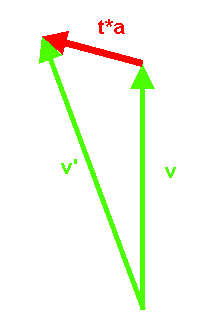
\includegraphics[width=0.5\linewidth]{figure2.png}
    \caption{Mouse movement for air strafing \cite{MoreSteamAirstrafe}}
\end{figure}

\section{Technical Background}


The main technical aspects of the bunny hop trainer revolve around emulating the physics engines present in Valorant and Counter-Strike that make bunny hopping possible. The main mechanic that makes movement acceleration possible is a technique called air strafing. While bunny hopping in a straight line is useful to keep the momentum of a player, air strafing is the main way in which players gain that increased momentum. Air strafing is performed by moving the mouse left, causing the player character to look left while holding the left movement key or looking right while holding the right movement key \cite{AirStrafingExplained}. Counter-Strike's movement engine, the source engine, is heavily based on the Quake movement engine and air strafing is a consequence of an interesting decision on how velocity and acceleration is calculated \cite{AirStrafingExplained}. Limiting player speed is important for controlling how a game will play as it dictates where players will encounter one another and limits the scope of engagements. Many games limit player speed by directly limiting velocity, ensuring that players can never reach greater speeds than the designers intended. In the Quake and Counter-Strike acceleration systems, only the projection of the current velocity onto acceleration is limited \cite{BunnyHoppingProgrammers}.


When pressing the movement keys in source games, the speed of the player is calculated each logical frame of the game. These logical frames are often called "ticks" and while a user can visually move locally in between ticks, their movement is only actually calculated every tick. Each logical frame, the game adds the acceleration vector in the direction the player's movement keys are being input to the player's current velocity vector \cite{BunnyHoppingProgrammers}. In order to keep the player's velocity below the speed limit, before applying the acceleration vector to the player each frame, the game calculates the vector projection with the acceleration added. Vector projection is the process of calculating the component of one vector that lies in the direction of another vector, represented by this equation: \[ V_{\text{proj}} = |\mathbf{a}| \cdot \cos(\theta) = \mathbf{a} \cdot \hat{\mathbf{b}} \] If this projection is greater than the speed limit, the acceleration is not added for that frame. By pressing the forward movement key in air, the projection of velocity will always be faster than the speed limit and thus acceleration will never be applied \cite{MoreSteamAirstrafe}. The only way that the character can gain velocity while staying under the speed limit is to accelerate directly perpendicular to the direction of movement. By moving the mouse as shown in figure 1, the character is gaining acceleration greater than the speed limit in the left direction \cite{MoreSteamAirstrafe}. By turning the mouse, the acceleration that would be going directly left and therefore not adding any forward velocity is now slightly below 90 degrees, and as such has a small forward component. This process is air strafing, moving the mouse slightly in one direction each frame to take advantage of the corresponding acceleration in that direction and convert some of that acceleration to forward acceleration.

\begin{figure}
    \centering
    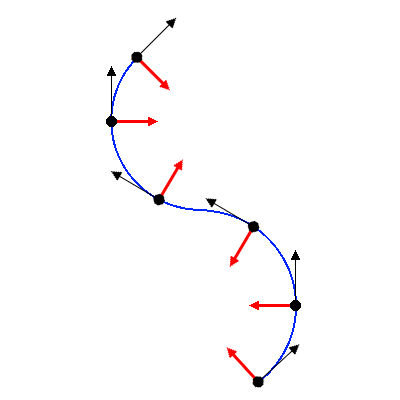
\includegraphics[width=0.5\linewidth]{figure1.png}
    \caption{Mouse movement for AD strafing \cite{MoreSteamAirstrafe}}
\end{figure}

Moving the mouse left while holding the left movement input gives some forward movement; however, in order to fully take advantage of air strafing for forward movement, the player must then follow this left movement with an equal right movement. Illustrated in figure 2, this process is commonly referred to as AD strafing because A is most commonly the left movement key and D is most commonly the right movement key. This technique of AD strafing keeps the player's acceleration always perpendicular to the velocity while fully taking advantage of the slight forward acceleration gain in both directions and although it looks confusing is the fastest way for a player to move in source engine games \cite{AirStrafingExplained}.

Other than emulating the acceleration and velocity, fully replicating the environment of a game engine is a difficult task. One of the main other mechanics that directly influences bunny hopping is friction. Bunny Hopping is a useful technique because friction is not calculated in the source engine on the first frame in which a player is in contact with the ground \cite{BunnyHoppingProgrammers}. Frames are fundamental units of time that represent individual snapshots of the game's state. Online multiplayer games like Counter-Strike have servers that take in input from all players in the game to calculate what is happening each tick. Counter-strike servers can calculate 64 tick per second while player's computers can render frames up to 240 times per second. The extra frames that the player's computer loads in between the server's logical ticks calculate a prediction of what each player will do and correct that prediction on receiving the next tick from the server \cite{MoreSteamAirstrafe}. Hitting the jump input on the exact frame in which a player touches the ground is very difficult and the main reason that bunny hopping is so difficult. One technique that players can use to make this easier is rebinding the jump key from the default space bar to a mouse wheel. Rolling the mouse wheel allows more inputs to be registered per second than possible by repeatedly pressing the space bar, in turn making the technique more consistent \cite{BhopTutorialValorant}.

In Counter-Strike 2, the most current version of Counter-Strike, and its predecessor Counter-Strike Global Offensive, bunny hopping has been made significantly more difficult and less effective. The velocity cap for Counter-Strike 2 is 330 HU (Hammer Units), which is much lower than previous games. In order to combat the use of the scroll wheel to consistently hit frame perfect bunny hops, Counter-Strike 2 has also implemented a server variable called sv\_jump\_spam\_penalty\_time which prevents the use of another jump input for a brief time after an input\cite{HowToBhopCS2}. This means that using the scroll wheel to send tens or hundreds of inputs will result in less consistency than manually using a jump input. Despite these handicaps, bunny hopping is still possible in Counter-Strike 2 but requires perfect inputs.


\section{Prior work}

% bunny rabbit 1999-06-03.md
Little academic work has been done on the mechanics of bunny hopping and air strafing, but there is a significant amount of non-academic research and documentation on the evolution of these techniques. Air strafing and bunny hopping was first discovered in the video game Quake and were mechanics that the lead developer did not like. In a series of archived blogs from the developer, John Carmack he says "In the absense of powerups or level features (wind tunnels, jump pads, etc), the game characters are supposed to be badasses with big guns. Arnold Schwartzenegger and Sigourney Weaver don't get down a hallway by hopping like a bunny rabbit." \cite{CarmackPlan} As this is one of the first documented times a bunny is mentioned in reference to the technique, this blog post may be the origin of bunny hopping as a term.
He even says "Strafe jumping is an exploitable bug. Just because people have practiced hard to allow themselves to take advantage of it does not justify it's existence." The only reason it stayed as a mechanic is "When I tried fixing the code so that it just didn't work, I thought it changed the normal running movement in an unfortunate way."\cite{CarmackPlan} This blog post was written a few months before the release of Quake III but shows that this foundational mechanic of fps games was initially a bug. This is also one of many times where game developers have attempted to remove bunny hopping from their games. This developer did successfully remove bunny hopping from sequels of Quake by removing air acceleration entirely \cite{bhopHistory}.
    
As explained in the technical background section, bunny hopping and air strafing exist due to the fundamental nature of the game's engine. Despite several attempts to "fix" bunny hopping, it took several games and several years to manage properly. Half-life 2 is another game on the source engine and contains bunny hopping. The developers attempted to remove bunny hopping by adding a negative velocity whenever the player reached a high enough acceleration. What they did not account for with this solution was bunny hopping backward. This oversight introduced the mechanic of Accelerated Back Hopping, which uses the negative velocity players gain from bunny hopping to reach speeds significantly higher than possible before \cite{ABH}.

The original Counter-Strike was a player made mod for the game Half Life in 2000 that included the bunny hopping present in the Quake engine, with a few minor tweaks. Counter-Strike made the movement slowdown from missing the frame perfect jump input more severe and added a movement speed cap to the player \cite{bhopHistory}. This version of bunny hopping was so popular that players created several types of maps that solely existed as obstacle courses for people to bunny hop through. Following Counter Strike was the release of Counter-Strike Source which was the first Counter-Strike game to use the source engine\cite{bhopHistory}. Counter-Strike source maintained none of the movement penalties for bunny hopping present in Counter-Strike and as such was a much less competitive game \cite{ExploringEsports}. The ability for players to move so quickly made designing a map with areas designed for players to encounter one another after a few seconds of walking was not possible, and players who mastered bunny hopping had significant advantages. Players who were not masters of the technique would become frustrated at players such as Phoon, a very talented player who recorded players irritation with his skill, and competitive matches of Counter-Strike were played on the previous version \cite{phoon}. Another problem with bunny hopping at this time was scripting. scripting is the process of running a computer script that perfectly executes a series of inputs allowing the player to bunny hop. While detection of these scripts is very good today, in the era of Counter-Strike Source, many players who were talented at bunny hopping were assumed to be cheaters \cite{bhopHistory}. 

Counter-Strike Global Offensive or CS:GO was the first instance where the developers really cracked down on bunny hopping. As the game began to accrue more of a competitive following, professional players and developers wanted to ensure that gameplay was intuitive and understandable. The maximum velocity was lowered and the punishment for missing a bunny hop was drastically increased \cite{HowToBhopCS2}. Bunny hopping in CS:GO and Counter-Strike 2 is more of a niche technique that can be used for bursts of speed instead of allowing the player to traverse the entire map as was possible in Counter-Strike Source.

Valorant was released in 2020, 8 years after the release of CS:GO and was designed to be a tactical shooter similar to CS:GO but easier to understand and interact with. The team built their engine from the ground up and this has allowed them more control over the mechanics present \cite{devDiaries}. Bunny hopping in Valorant is significantly easier than it is in Counter-Strike as there is no slowdown penalty for missing the frame perfect input of the jump. However, bunny hopping does not allow the player to move any faster than normal speed and is primarily used as an evasion technique or in combination with air strafing to retreat behind cover more quickly \cite{BhopTutorialValorant}. Air strafing in valorant is also unaffected by usage of the W key, making it much more intuitive than Counter-Strike air strafing.

Many Youtube videos exist that teach users how to bunny hop across various games. There are tutorials for Quake, Valorant, and all iterations of Counter-Strike. Most of these tutorials follow a similar general structure. The player will introduce the technique with a flashy clip showing its usefulness, then explain how to airstrafe and how to bunny hop \cite{QuakeBHopTutorial}. Often these guides will also give the user a helpful place to practice in game. While these tutorials are helpful, many of them are lacking important context and feedback necessary in understanding the skill. Almost all of these tutorials mention "moving the mouse smoothly" for air strafing, which is useful but does not explain to the user the processes that are occurring and why smooth movement is important \cite{HowToBhopCS2}. The change in angle of the mouse movement is more important than the smooth movement, but in a video format is difficult to portray \cite{BhopTutorialValorant}. Many tutorials will also include statements like "as you can see its actually pretty easy," which can make the player discouraged if the technique is not as easy for them to learn \cite{QuakeBHopTutorial}. Some tutorials include visualizations of what keys are being pressed by the player, which is helpful but visualizing mouse movement is significantly more difficult and is a lacking component of most tutorials. These shortcomings of the video format are all solvable with an interactive player controlled trainer.

Aim Lab is a widely used "aim trainer" tool that allows players to practice their mouse aim by shooting virtual targets. Each scenario is typically one minute long and the goal of the activity is to hit as many targets as possible while keeping their accuracy as high as possible. This technique of isolated practice of a single aspect of a game is a large inspiration for this project and has shown to be widely used in the gaming space with 30 million players \cite{STEAMDBAimLabChart}. This technique has proved to be effective as it allows users to more quickly build muscle memory for aiming and helps train the aiming motor pathway \cite{aimTrainingWorks}. Aim Lab also gives users feedback on each task they complete and if the user is struggling with a certain aspect of their aim will suggest scenarios to train that aspect. The user feedback also gives encouraging statistics to players, congratulating them on their improvements and finding positives in their failures.


\section{Ethical Considerations}

While the goal of this project is to make an advanced technique in first person shooter games more accessible to a wide variety of people, it is important to recognize the lack of accessibility in some parts of the project. Video games are often created with a control schema that matches the developer's own ability, and many lack flexibility in gameplay options. For someone who is blind, a game that entirely relies on visual feedback is impossible to interface with. While a blind person is a clear example of someone who will struggle to use this tool, the way in which it is designed will make it difficult for people with a wide variety of limiting conditions. Despite being a tool intended to teach those with all levels of familiarity, the reliance on text prompts to relay information and data on the success of the user in the task is also a significant hurdle\cite{AccessInVidya}. Including the option for audio instruction and feedback could make the game more accessible to those with dyslexia or who are not literate. 

First-person shooters are very difficult to make accessible. Since the bunny hop trainer is a tool for teaching skills used in a first-person shooter, these accessibility concerns are inherited. As presented in the initial proposal, there is no support for controller input or any input that is not a keyboard and a mouse. Alternative input devices can be helpful tools for those who do not have the full ability to use traditional control schemes. For many people with accessibility concerns, a one-handed controller can often allow them to play a game they would not otherwise be able to. One-handed controllers are very difficult to implement for first-person shooters because they require two analog inputs simultaneously, one to control the player's movement and one to control the player's aim \cite{GameAccesibilityASurvey}. Other controllers, such as brain wave or eye-tracking controllers, are also difficult to implement for first-person shooters due to the precise nature of aiming with the mouse that it is trying to replicate. Even for those who have the ability to interface with a keyboard and mouse, the precise nature of the movements required to execute an air strafe with a mouse will further limit their ability to interface with the tool. While adding controller support would make the trainer far more accessible, Valorant and Counter-Strike are both games that do not have native support for controllers and adding this support would be a considerable undertaking. Air strafing is also requires discrete left and right inputs which are significantly harder to execute on an analog controller thumb stick. Bunny hopping is also not a necessary skill to play Counter-strike or Valorant and, in the vast majority of cases, is nothing more than a flashy technique that has no impact on the game. For these reasons I have decided not to add controller support to the first iteration of this tool.

\section{Methods}

The goal of this project is to create an app that trains new users to successfully and consistently perform air strafes and bunny hops in Valorant and Counter-Strike 2. This app will be developed in Unity and guide the player through the mechanics of bunny hopping step by step, giving qualitative feedback on the user's performance. The first thing that I will focus on for this project is developing a game environment in Unity that accurately replicates Counter-Strike 2 and a game environment that replicates Valorant. Several tutorials and premade environments exist that I will use to emulate the game as closely as possible. Counter-Strike offers tools that show how quickly the player moves in game. I plan to gather data from Counter-Strike on the amount of time it takes a player to travel a certain distance and use the same Counter-Strike map in the Unity engine to ensure my values for acceleration, velocity, jump height and gravity are in line with the game. I plan to follow a similar process for Valorant as both these games have map assets that are freely available. 

After replicating the game environment, I will create the system to give user feedback. I will begin by creating the bunny hop timing scenario, where the user will perform a number of bunny hops and the application will tell them how accurately they performed the movement and what they can do to improve. This user feedback is inspired by Aim Labs and other similar aim trainer tools discussed earlier. After designing the bunny hop scenario, I will design the air strafe scenario. This scenario starts with instructing the user to move their mouse smoothly at the appropriate angle and will provide feedback on how far off the optimal angle they were and whether they were too fast or too slow. After this initial stage, the user will be instructed to add in AD strafing and will receive feedback on how closely their key strafes matched their mouse movement. Lastly for user feedback I will implement a scenario that brings all these components together into a full bunny hop scenario. The feedback for this scenario will be simplified to jump consistency and overall forward velocity with indicators of goals for each. I will also build a system that records previous results and encourages users by showing them their improvement and allows them to see their progress.

\section{Evaluation metrics}

The goal of this project is to create a tool that allows users to learn how to bunny hop or improve their consistency with that skill. The goal for evaluations will be to see the impact of the tool in these games. Counter-Strike allows users to create their own maps with functional elements inside so for Counter-Strike I will develop a map with a straight area that times how long users spend between two trigger zones and also records the velocity of the player. For Valorant, which does not have this functionality, I will have users enter a custom game and have another player record their perspective from above and calculate the time it takes users to cross between two points. I will have all participating testers of the tool attempt to bunny hop 5 times in their corresponding game environment before they begin using the tool and again after three days and a week of using the tool for 20 minutes a day. If there is a meaningful change in the amount of time it takes a user on average to cross the distance while bunny hopping then my tool is effective. 

The goal for my testing is to run multiple week long tests with different users of different skill levels. Finding users who will be willing to participate in a week long test may be difficult but ideally I would want at least four new users for each game who are learning to bhop for the first time and two users for each game who have some familiarity with bunny hopping. The goal of this tool is primarily to teach new players how to bunny hop, but I would also like to see the potential impact on improving the consistency of players who already possess the technique.

The other goal for user testing is to ensure that the application is as user-friendly as possible and is a tool that people will actually use in the future. I will run one shorter test entirely focused on getting user feedback for usability and in the test for project results I will also request that users fill out a short survey about what they feel could be improved. The survey questions will be as follows:
\begin{enumerate}
    \item What is your pre-existing familiarity with bunny hopping?
    \item Do you feel this tool was helpful for learning how to bunny hop?
    \item Is this a tool you would use outside of this study?
    \item What would make this tool easier to use?
    \item If you could add one feature to this tool what would it be?
    \item Did this tool improve your confidence with bunny hopping?
    
\end{enumerate}

\section{Timeline}

My proposed timeline for this project is as follows:
\textbf{May 1-15:}
Create the comps proposal and research the problem domain.

\textbf{May 15-July 15:}
Do more research on the Unity engine and practice creating environments for other projects. I will also consistently practice bunny hopping so that I can appropriately test if my game environments replicate the real game.

\textbf{July 15-August 23:}
Continued practice of bunny hopping and evaluation of trainer tools that exist to teach people mechanics.

\textbf{August 23-September 15:}
Begin work on the central component for the project, main goal for this period is to have a functional and accurate unity environment that replicates Counter-Strike 2. I also plan to begin searching for users who would be appropriate test subjects for this project.

\textbf{September 15- September 30:}
Goal for this period is to have a functional and accurate unity environment for Valorant and to build both the bunny hop timing tracker and the mouse angle movement tracker. With these core mechanics built I will be able to prepare users for testing

\textbf{October 1 - October 15:}
In this period the goal is to have a functional rough version of the application that gives users feedback on their mechanics. I plan to have the first round of user testing take place with a primary focus on improving the application, not measuring results.

\textbf{October 15 - October 31:}
In this period I will improve the user experience with the application and develop the testing protocols for in-game experience with a custom Counter-Strike map and a set protocol for recording Valorant speed in game. At the end of this period I plan to record initial user data before using my tool and begin the user testing.

\textbf{November 1 - November 15:}
In this period I will assist users in using the application and record their progress. After this I will interpret the user's data and determine wether or not my application is helpful. If the poster is still due during this period I will start and complete the poster, otherwise I will spend this time starting the poster.

\textbf{November 16 - November 30:}
I will spend this time fully refining the application. I plan to significantly improve the user interface and flesh out the user feedback section by adding positive messages and allowing the user to check on their progress. If still possible I will work on my poster and practice presenting it. I will also make a version of the project that is publicly available if people want to try it.

\textbf{December 1 - December 15:}
This period of time will be spent exclusively on finishing the COMPS paper and if necessary fixing any bugs that arise from greater user testing. This period will also be spent working on other classes and seeing as the project should hopefully be close to completion this section should not take much time.
 



    

\printbibliography

\end{document}
